%!TEX root = ../main.tex
% !TeX spellcheck = en_GB 


\chapter{Results}
\section{Overtaking and head-on situation}
\begin{figure}[H]
    \centering
    \includegraphics[width=\textwidth,height=0.75\textheight,keepaspectratio]{Figures/Scenario/overtaking-and-head-on-res.pdf}
    \caption{Overtaking and head-on situation on the high seas }
    \label{fig:overtaking-and-head-on-res}
\end{figure}
\section{Overtaking and crossing situation}

\begin{figure}[H]
    \centering
    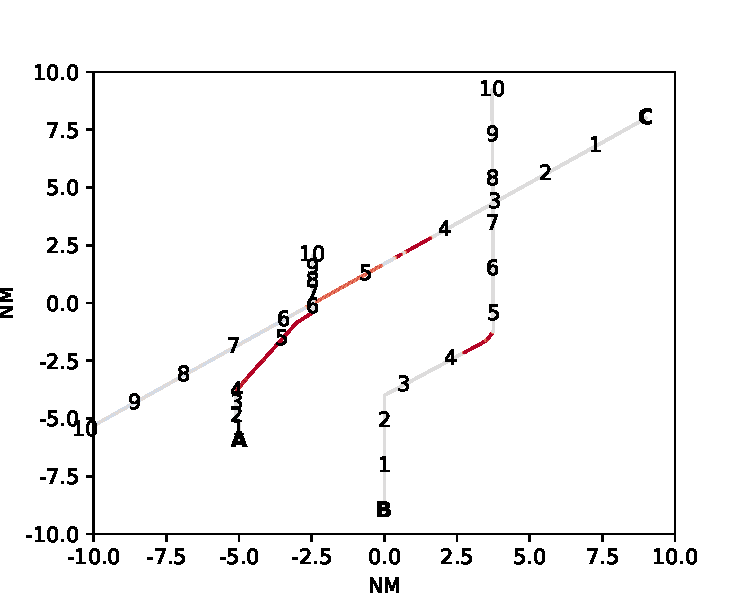
\includegraphics[width=\textwidth,height=0.75\textheight,keepaspectratio]{Figures/Scenario/overtaking-and-crossing-res.pdf}
    \caption{Overtaking and crossing situation}
    \label{fig:overtaking-and-crossing-res}
\end{figure}
\begin{figure}[H]
    \centering
    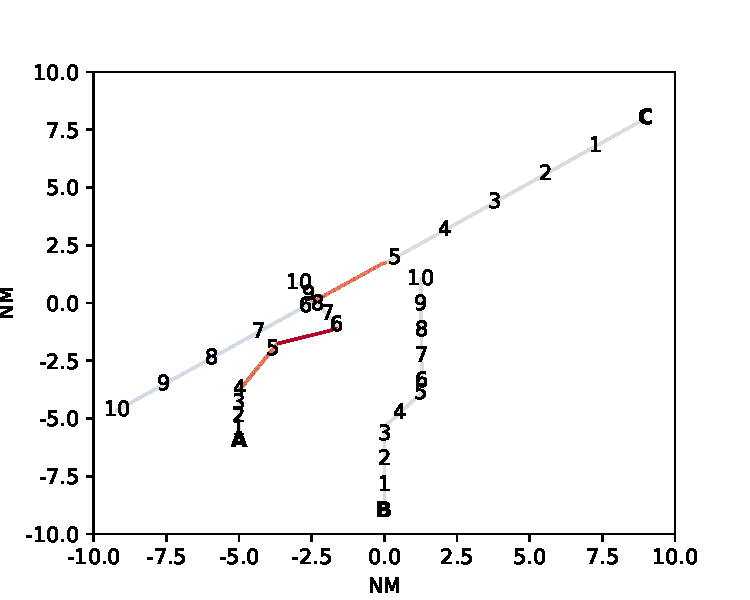
\includegraphics[width=\textwidth,height=0.75\textheight,keepaspectratio]{Figures/Scenario/overtaking-and-crossing-3-res.pdf}
    \caption{Overtaking and crossing situation }
    \label{fig:overtaking-and-crossing-3-res}
\end{figure}
\begin{figure}[H]
    \centering
    \includegraphics[width=\textwidth,height=0.75\textheight,keepaspectratio]{Figures/Scenario/overtaking-and-crossing-2-res.pdf}
    \caption{Overtaking and crossing situation }
    \label{fig:overtaking-and-crossing-2-res}
\end{figure}

\chapter{Discussion}
\chapter{Conclusion}